% This document is compiled using pdfLaTeX
% You can switch XeLaTeX/pdfLaTeX/LaTeX/LuaLaTeX in Settings

\documentclass{article}
\usepackage{ctex}
\usepackage{csquotes} % 对于智能引用符号
\usepackage[backend=biber,style=numeric]{biblatex} % 使用biblatex和biber
\usepackage{geometry}
\usepackage{graphicx}
\usepackage{listings}
\usepackage{minted}
\usepackage{amsmath}
\usepackage{amsfonts}
\usepackage[T1]{fontenc}
\usepackage{lmodern}
\usepackage{amssymb}
\usepackage{marginnote}
\usepackage{xcolor}
\usepackage{hyperref}
\usepackage{todonotes}
\usepackage[utf8]{inputenc}
\usepackage{url} % 加载url包

% 设置页边距
\geometry{
    left=1.5cm,         % 左边距
    right=3cm,        % 右边距
    top=2.5cm,          % 上边距
    bottom=2.5cm        % 下边距
}

\lstset{
  language=Python,      % 语言类型
  basicstyle=\tt, %使用teletype字体
}

% 添加参考文献文件
\addbibresource{references.bib}

\title{异构图增强对比学习:基于\emph{ReChorus}框架的复现实验}
\author{中山大学人工智能学院\quad 苏睿熹\quad 詹宇涵}
\date{}

\begin{document}
\begin{minipage}[t]{\textwidth}
    \vspace{-0.5cm}
    \begin{center}
        \vspace{-1.5cm} % 减少间距
        
\includegraphics[width=0.2\textwidth]{sysu.jpg}\\
        \vspace{-1.5cm} % 减少间距
    \end{center}
    \maketitle
\end{minipage}

\section{项目背景}

本项目为中山大学人工智能学院2022级机器学习课程的作业,主要工作为利用\emph{ReChorus}框架\cite{wang2020make}对异构图增强对比学习(Heterogeneous Graph Contrastive Learning,\emph{HGCL})\cite{Chen_2023}进行复现。该项目已在 \lstinline{gitee} 上开源:\url{git@gitee.com:su-ruixi/HGCL_ReChorus_SYSU.git}。

\subsection{\emph{HGCL}异构图增强对比学习}

在推荐系统中,图神经网络(\emph{GNN})已经成为处理图结构数据的强大工具。图神经网络能够成功地编码用户和项目之间的关系\cite{Wu_2022},其核心是通过跨图传播层聚合相邻特征信息来学习节点(用户或项目)的表示。许多基于图神经网络的协同过滤(\emph{CF})模型只关注生成的useritem连接图中的同构交互关系\cite{Chen_2020,he2020lightgcnsimplifyingpoweringgraph,Wang_2019}。然而,在现实世界的推荐场景中,异构关系信息无处不在\todo[size=\small, color=pink]{异构关系是指在推荐系统中用户与项目之间存在多样性和复杂性的交互作用,包括但不限于用户的社会网络连接和基于知识的项目依赖关系,这些关系携带丰富的语义信息,有助于提高推荐系统的性能。}(例如用户的社会影响力,项目之间的知识依赖性),这些关系包含了大量的信息来增强用户偏好的学习。当前的异构图神经网络是标签数据密集型学习模型,因此可能无法生成具有稀疏交互标签的高质量用户/项目嵌入用于推荐系统的模型优化\cite{Long_2021,Wu_2021}。最近,对比自监督学习在推荐领域取得了成功,这为通过不同视角间的知识转移来改进用户与项目互动模型提供了一种新途径。

异构图增强对比学习(\emph{HGCL})\cite{Chen_2023}基于图神经网络和对比自监督学习,将异质关系语义整合到用户与项目互动建模中,并通过对比学习增强的知识转移跨越不同的视图。由于异质侧信息对用户和项目交互的影响可能会有所不同,\emph{HGCL}使用元网络增强,使得可以进行个性化的知识转换,并提供适应性的对比增强从而使得模型效果更优。

\subsection{\emph{ReChorus}框架}

\emph{ReChorus}框架是一个基于PyTorch构建的综合、高效、灵活且轻量级的推荐算法框架\cite{wang2020make},旨在为推荐算法的研究人员提供一个统一的基准来实现和比较各种算法。\emph{ReChorus}通过分离算法共性和特性部分的设计思想,实现了包括经典推荐方法以及最新基于深度学习的推荐模型在内的多种推荐算法,并通过读取(Reader)、运行(Runner)、模型(Model)三大模块整合了数据处理、模型训练与评估等功能。该框架不仅在确保综合性和高效性的基础上保持了轻量化和实用性,而且具有很好的扩展性。本文将阐述基于此框架复现\emph{HGCL}的详细过程。

\section{理论:\emph{HGCL}建模与分析}

该部分将介绍异构图增强对比学习的模型架构及其逻辑。

\subsection{模型架构}

\emph{HGCL}框架由三个核心部分组成:第一部分,利用异构图神经网络在用户—用户图、用户—项目图和项目—项目图上进行异构图的提取与融合;第二部分,设计了一个元网络用于建模辅助视图与交互视图之间的个性化跨视图依赖关系;第三部分,通过异质关系视图间的自适应对比学习来进行联合参数优化。这样的设计使得模型能够在推荐系统中有效地结合异构侧信息,并且通过对比学习增强知识传递,从而提高推荐准确性。其框架图 1如下所示。

\begin{figure}[htbp]
    \centering
    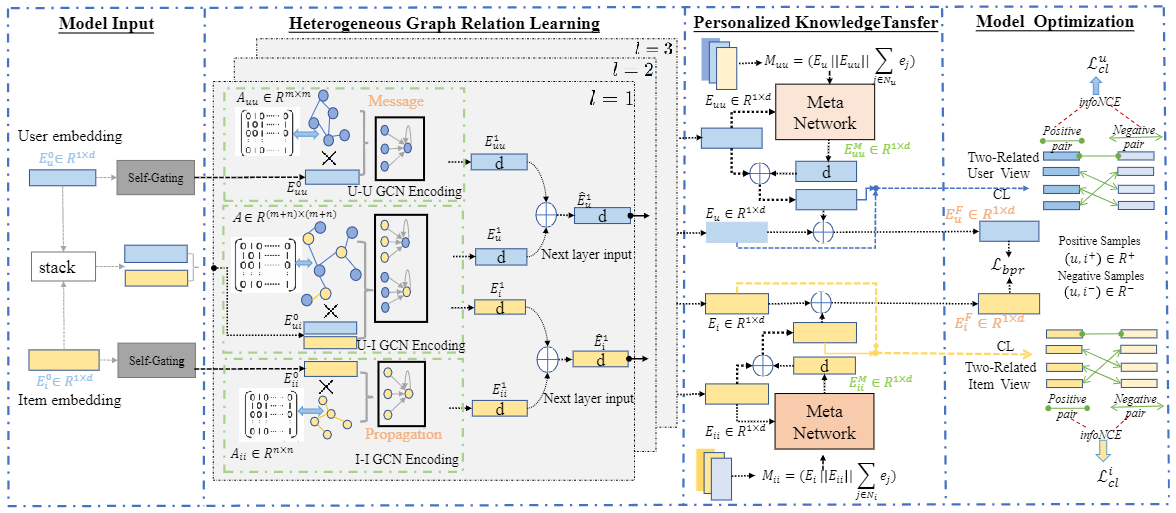
\includegraphics[width=1\textwidth]{figure1.png}
    \caption{\emph{HGCL}框架图示\cite{Chen_2023}}
    \label{fig:your_image_label}
\end{figure}

\subsection{\emph{Heterogeneous Graph Relation Learning}异构图关系学习}

\subsubsection{信息嵌入与提取}

\emph{HGCL}基于推荐系统中的用户—项目交互、用户间社会关系以及项目间关联三种异质关系,定义了图结构($G_{ui}$,$G_{ii}$和$G_{uu}$)及对应的衔接矩阵($A_{ui}$,$A_{ii}$和$A_{uu}$)。并使用异构图神经网络,进行关系感知嵌入初始化工作。

具体地,\emph{HGCL}使用Xavier初始化器\todo[size=\small, color=pink]{Xavier初始化器是一种用于神经网络权重初始化的技术,它通过调整初始权重的规模来帮助加速深层网络的训练,并促进更稳定的梯度流动。}\cite{pmlr-v9-glorot10a}为每个节点分配id相应的嵌入$\mathbf{e}_u,\mathbf{e}_i\in\mathbb{R}^d$,其中$d$表示隐藏维度。这些节点特异性嵌入形成初始嵌入矩阵$\mathbf{E}_{ui}^0\in\mathbb{R}^{m\times d}$和$\mathbf{E}_i^0\in\mathbb{R}^{n\times d}$。将初始嵌入馈送到用户—项目域、用户—用户域和项目—项目域的不同图编码器中。

\emph{HGCL}通过训练一个带有乘法跳跃连接\cite{pmlr-v70-dauphin17a}的自控门模块\cite{yu2022selfsupervisedmultichannelhypergraphconvolutional},来刻画三种关系的交互模式差异。其从共同的初始嵌入空间中推导出关系感知嵌入,如下所示:
\begin{equation}
\mathbf{E}_{uu}^0 = \mathbf{E}_u^0 \odot \sigma(\mathbf{E}_u^0\mathbf{W}_g+\mathbf{b}_g); \quad \mathbf{E}_{ii}^0 = \mathbf{E}_i^0 \odot \sigma(\mathbf{E}_i^0\mathbf{W}_g+\mathbf{b}_g)
\end{equation}

其中$\mathbf{E}_{uu}^0\in\mathbb{R}^{m\times d}$和$\mathbf{E}_{ii}^0\in\mathbb{R}^{n\times d}$分别是用户级和项目级关系的同构图$G_{uu}$和$G_{ii}$的嵌入。$\sigma(\cdot)$表示Sigmoid激活函数。$\odot$表示元素乘法操作。$\mathbf{W}_g\in\mathbb{R}^{d\times d}$和$\mathbf{b}_g\in\mathbb{R}^{d\times 1}$是变换和偏差参数。
该模块使得嵌入$\mathbf{E}_{uu}^0,\mathbf{E}_{ii}^0$不仅与用户—项目交互的初始嵌入$\mathbf{E}_u^0,\mathbf{E}_i^0$共享语义,还获得了刻画用户—用户和项目—项目关系的灵活性。

\subsubsection{信息融合与聚集}

\emph{HGCL}将图卷积神经网络作为三个图结构视图的编码器。初始嵌入矩阵中的$\mathbf{E}_u^0,\mathbf{E}_i^0$作为用户—项目视图的输入,$\mathbf{E}_{uu}^0$和$\mathbf{E}_{ii}^0$分别作为用户—用户视图和项目—项目视图的输入。给定用户—项目交互图$G_{ui}$,\emph{HGCL}通过以下的消息传递进行迭代细化:
\begin{equation}
    \mathbf{e}_u^{l+1}=\sum_{i\in\mathcal{N}_u}\frac{1}{\sqrt{|\mathcal{N}_u|}\sqrt{|\mathcal{N}_i|}}\mathbf{e}_i^l; \quad \mathbf{e}_i^{l+1}=\sum_{u\in\mathcal{N}_i}\frac{1}{\sqrt{|\mathcal{N}_i|}\sqrt{|\mathcal{N}_u|}}\mathbf{e}_u^l
\end{equation}

其中$\mathcal{N}_u$和$\mathcal{N}_i$分别表示目标节点$u$和$i$的邻居集。$\mathbf{e}_u^l,\mathbf{e}_i^l\in\mathbb{R}^d$是在第$l$次迭代时用户$u$和项目$i$的嵌入向量。$\mathbf{e}_u^0,\mathbf{e}_i^0$分别是嵌入矩阵$\mathbf{E}_u^0,\mathbf{E}_i^0$的行向量。受轻量级GCN\cite{he2020lightgcnsimplifyingpoweringgraph}的启发,\emph{HGCL}的关系感知消息传递范式没有配置变换和非线性激活。同样,$\mathbf{E}_{uu}^L$和$\mathbf{E}_{ij}^L$也是按照相同的方式迭代。

\emph{HGCL}受\emph{HGT}\cite{hu2020heterogeneousgraphtransformer}中soft meta-path的启发,每轮迭代的信息来自异构关系的聚集。通过异构消息传递的多次迭代,高阶嵌入将保持具有多跳连接的异构语义。用户和项目的嵌入的更新如下:
\begin{equation}
\widehat{\mathbf{E}}_u^{l+1}=f(\mathbf{E}_u^{l+1},\mathbf{E}_{uu}^{l+1}); \quad \widehat{\mathbf{E}}_i^{l+1}=f(\mathbf{E}_i^{l+1},\mathbf{E}_{ii}^{l+1})
\end{equation}

其中嵌入$\widehat{\mathbf{E}}_u^{l+1}\in\mathbb{R}^{m\times d}$和$\widehat{\mathbf{E}}_i^{l+1}\in\mathbb{R}^{n\times d}$整合了第$l+1$层的异构语义中,作为下一层的输入。$f$表示使用元素平均池化的异构信息融合函数\todo[size=\small, color=pink]{元素平均池化是一种在处理多通道或多重表示时使用的聚合技术,通过对各个元素求平均值来融合不同来源的信息。}。
为进一步综合编码后的各层表示($1\leq l\leq L$),\emph{HGCL}按如下方式生成用户—项目的整体嵌入:
\begin{equation}
\mathbf{E}_u=\mathbf{E}_u^0 + \sum_{l=1}^L\frac{\mathbf{E}_u^l}{||\mathbf{E}_u^l||}; \quad \mathbf{E}_i=\mathbf{E}_i^0 + \sum_{l=1}^L\frac{\mathbf{E}_i^l}{||\mathbf{E}_i^l||}
\end{equation}

其中$L$表示GCN迭代的最大次数。每一层GCN的输出都进行了归一化。用户—用户社交视图(即$\mathbf{E}_{uu}$)和项目—项目依赖视图(即$\mathbf{E}_{ii}$)的整体嵌入以类似的方式获得。

\subsection{\emph{Cross-View Meta Network}跨视图元网络设计}

在现实的用户建模场景中,用户和项目的侧面信息对用户—项目交互模式的影响可能因人而异。为了进行个性化的知识转移,从侧面信息引导特定用户的偏好学习。\emph{HGCL}设计了一个跨视图元网络,以实现来自用户和项目侧面的定制化知识蒸馏。

\subsubsection{元知识提取}

为了从辅助视图(用户和项目的侧面信息)生成到每个用户和每件项目的用户—项目交互编码的个性化映射,\emph{HGCL}首先提取元知识以保留与辅助视图和交互视图相关的用户和项目的重要特征。具体来说,用户—用户关系视图和项目—项目关系视图的蒸馏元知识如下获得:
\begin{equation}
\mathbf{M}_{uu}=\mathbf{E}_u||\mathbf{E}_{uu}||\sum_{i\in\mathcal{N}_u}\mathbf{e}_i;\quad\mathbf{M}_{ii}=\mathbf{E}_i||\mathbf{E}_{ii}||\sum_{u\in\mathcal{N}_i}\mathbf{e}_u
\end{equation}

其中 \( \mathbf{M}_{uu} \in \mathbb{R}^{m \times 3d}, \mathbf{M}_{ii} \in \mathbb{R}^{n \times 3d} \) 表示元知识,分别编码上下文信息以生成用户侧和项目侧知识的个性化知识转移函数。受到\cite{Xia_2021}的启发,元知识包含了源域(即用户—用户和项目—项目关系视图)的节点表示 \( \mathbf{E}_{uu}, \mathbf{E}_{ii} \),以及目标用户—项目交互视图的嵌入 \( \mathbf{E}_u, \mathbf{E}_i \)。此外,我们将邻接信息纳入元知识中。

具体来说,辅助域的嵌入表征了用户的社交影响力和项目语义相关性。用户—项目视图的嵌入捕捉了用户的项目相关互动模式。附加的邻接信息明确增强了直接图连接的建模。通过综合考虑这三个维度的信息,元知识能够很好地反映个性化跨视图知识传递的重要上下文信号。

\subsubsection{个性化的跨视图知识转移}

\emph{HGCL}将提取出的元知识用来生成带有变换矩阵的知识转移网络,其元神经网络如下所示:
\begin{equation}
\begin{cases}f_{mlp}^1(\mathbf{M}_{uu})\to\mathbf{W}_{uu}^{M1}\\f_{mlp}^2(\mathbf{M}_{uu})\to\mathbf{W}_{uu}^{M2}\end{cases}
\end{equation}

其中 \( f_1^{mlp}, f_2^{mlp} \) 是包含两个带有PReLU激活函数的全连接层的元知识学习器。这些函数以元知识 \( \mathbf{M}_{uu} \) 作为输入,并输出定制的变换矩阵 \( \mathbf{W}_{uu}^{M1} \in \mathbb{R}^{m \times d \times k},\mathbf{W}_{uu}^{M2} \in \mathbb{R}^{m \times k \times d} \)。

这两个参数张量各自包含 \( m \) 个矩阵,对应于每个用户。根据相应用户和项目的独特特性来生成定制的转换,从而实现个性化的知识转移。两组矩阵将变换的秩限制为 \( k<d \),这不仅减少了元知识学习者的可训练参数数量,而且增强了模型的稳定性。受个性化桥接函数\cite{Xia_2021}的启发,我们利用生成的参数矩阵和一个非线性映射函数来构建我们的定制传输网络如下:
\begin{equation}
\mathbf{E}_{uu}^M=\sigma(\mathbf{W}_{uu}^{M1}\mathbf{W}_{uu}^{M2}\mathbf{E}_{uu})
\end{equation}

其中 \( \sigma(\cdot) \) 表示PReLU激活函数\todo[size=\small, color=pink]{PReLU是一种激活函数,它在ReLU的基础上加入了线性斜率参数,使得神经元在负区间也有非零的导数,从而可以更好地解决梯度消失问题并加速收敛。}。\( \mathbf{E}^{\text{Mu}} \in \mathbb{R}^{m \times d} \) 包含由自定义映射函数对用户—用户社交视图进行转换后的嵌入。然后使用自定义嵌入增强来自用户—项目交互编码的用户嵌入。对于用户的融合过程是通过以下加权求和完成的:
\begin{equation}
    \mathbf{E}^F_u = \alpha_u * \mathbf{E}_u + (1 - \alpha_u) * (\mathbf{E}_{uu} + \mathbf{E}^M_{uu})
\end{equation}

其中 \( \alpha_u \in \mathbb{R} \) 表示控制用户—项目交互视图嵌入和用户—用户社交视图嵌入之间的权重。\( \mathbf{E}^F_u \in \mathbb{R}^{m \times d} \) 表示用于主要推荐任务的最终嵌入。跨视图项目嵌入 \( \mathbf{E}^M_{ii}, \mathbf{E}^F_i \) 可以以类似的方式生成。

\subsection{\emph{Heterogeneous Graph Contrastive Learning}异构关系对比学习}

该部分为本模型的关键,对应于模型框架的第三部分。

\subsubsection{跨视图对比学习}

为了进一步增强框架的表示学习,\emph{HGCL}引入更多的监督信号来缓解数据稀疏性问题,设计了跨视图对比学习范式。通过两个辅助视图(即 \( \mathbf{E}^M_{uu} \) 和 \( \mathbf{E}^M_{ii} \))的嵌入与用户—项目交互视图(即 \( \mathbf{E}_u \) 和 \( \mathbf{E}_i \))的嵌入对齐,辅助视图的嵌入作为有效的正则化影响用户—项目交互建模的自监督信号。

考虑到个性化的跨视图知识转移,\emph{HGCL}结合了个性化跨视图知识转移和对比学习。特别是,在不同表示视图之间以自适应方式执行跨视图嵌入对齐。特定于辅助视图的嵌入 \( \mathbf{E}_{uu}, \mathbf{E}_{ii} \) 通过元网络生成的个性化映射函数处理,产生个性化的辅助嵌入 \( \mathbf{E}^M_{uu}, \mathbf{E}^M_{ii} \)。元网络经过训练,可以过滤掉辅助视图中的噪声特征,以匹配用户—项目交互视图。

\subsubsection{基于InfoNCE的对比损失}

借助我们的异构图关系学习和跨视图元网络,我们获得了用户和项目的两组嵌入,即对于用户有 $\mathbf{E}^{M}_{uu}$, $\mathbf{E}_u$,对于项目有 $\mathbf{E}^{M}_{ii}$, $\mathbf{E}_i$。这些嵌入是通过对用户-项目交互数据及用户/项目侧辅助知识进行编码获得的。受到最近对比自监督学习在推荐领域成功应用的启发\cite{Wu_2021}\cite{Xia_2022},我们提出使用基于InfoNCE的对比学习损失来增强我们HGCL方法在两个表示视图之间的用户/项目表示学习,公式如下:
\begin{equation}
\mathcal{L}_{cl}^u=\sum_{u\in\mathcal{V}_u}-\log\frac{\exp\left(s(\mathbf{e}_{uu}^M+\mathbf{e}_{uu},\mathbf{e}_u)/\tau\right)}{\sum_{u^{\prime}\in\mathcal{V}_u}\exp\left(s(\mathbf{e}_{uu}^M+\mathbf{e}_{uu},\mathbf{e}_u^{\prime})/\tau\right)}
\end{equation}

其中,$\mathbf{e}^{Mu}_{u} \in \mathbb{R}^d$, $\mathbf{e}_u \in \mathbb{R}^d$ 分别是从矩阵 $\mathbf{E}^{M}_{uu}$ 和 $\mathbf{E}_u$ 中的嵌入向量。$s(\cdot)$ 表示相似度函数,它可以是内积或余弦相似度。这里我们采用余弦相似度作为 $s(\cdot)$。$\tau$ 代表温度系数,它能够自动识别困难的负样本。$u'$ 表示具有不同索引的负样本。

类似地,我们可以得到项目方面的InfoNCE损失 $L^{cl}_i$。
最终,总的对比损失为 $L^{cl} = \alpha_1 * L^{cl}_u + \alpha_2 * L^{cl}_i$,其中 $\alpha_1$ 和 $\alpha_2$ 是用于权重调整的超参数。

\subsection{\emph{HGCL}的优化目标}

使用融合嵌入 \( \mathbf{E}^F_u, \mathbf{E}^F_i \),我们的\emph{EGCL}预测用户 \( u \) 与项目 \( i \) 交互的概率 \( \hat{y}_{u,i} = \mathbf{e}^F_u \mathbf{e}^F_i \),其中 \( \mathbf{e}^F_u \) 和 \( \mathbf{e}^F_i \) 分别表示融合嵌入矩阵中的最终用户 \( u \) 和项目 \( i \) 的嵌入向量。\( \hat{y}_{u,i} \in \mathbb{R} \) 表示用户 \( u \) 与项目 \( i \) 交互的可能性分数。较大的 \( \hat{y}_{u,i} \) 表明交互概率较大。为了优化推荐任务下的\emph{HGCL},我们遵循近期工作并采用Bayesian Personalized Ranking (\emph{BPR})\cite{rendle2012bprbayesianpersonalizedranking}对比损失函数。具体来说,每个训练样本配置了一个用户 \( u \),一个用户已交互的正面项目 \( i^+ \),以及一个用户未交互的负面项目 \( i^- \)。对于每个训练样本,我们最大化预测得分如下:
\begin{equation}
\mathcal{L}_{bpr}=\sum_{(u,i^+,i^-)\in O}-\ln(\mathrm{sigmoid}(\hat{y}_{u,i^+}-\hat{y}_{u,i^-}))+\lambda||\Theta||^2
\end{equation}

其中 $\ln(\cdot)$ 和 \( \mathrm{sigmoid}(\cdot) \) 分别表示对数函数和Sigmoid函数。\( \lambda \) 表示确定正则化项权重的超参数。将 BPR 损失函数与增强的跨视图对比学习损失相结合,整体训练损失如下:
\begin{equation}
\mathcal{L} = \mathcal{L}_{bpr} + \beta * \mathcal{L}_{cl}
\end{equation}

\section{实验:基于\emph{ReChorus}框架的复现过程}

本部分将尽可能详细地展示基于\emph{ReChorus}框架的对\emph{HGCL}复现过程。

\subsection{环境配置}

\emph{ReChorus}框架的配置过程如下Listing 1所示。

\begin{lstlisting}[language=Python,caption=环境配置]
! conda create -n ReChorus python=3.10.4
! conda activate ReChorus
IN requirements.txt: 
    delete torch==1.12.1, pickle #pickle为python=3.10自带,torch需要用pip安装
    turn numpy==1.22.3 to numpy==1.23.5 #调整numpy版本适配scipy库
conda install --file requirements.txt
pip install torch==1.12.1
\end{lstlisting}

\subsection{数据处理}

在\emph{HGCL}的工作\cite{Chen_2023}中采用了\lstinline{CiaoDVD}\cite{guo2014etaf}等三个评分数据集进行实验。其原始数据输入包含:
\begin{itemize}
    \item \lstinline{rating.mat}: 包含用户对项目的评分数据,每行记录用户ID、物品ID、类别ID和评分。
    \item \lstinline{trust.mat}: 描述用户之间的信任关系,每行记录一个信任用户ID和被信任用户ID。
\end{itemize}

然而,在\emph{ReChorus}框架中使用的数据集(\lstinline{Grocery_and_Gourmet_Food},\lstinline{MIND-Large} 和 \lstinline{MovieLens-1M})里并未提供关于描述用户之间信任关系(who-trust-who)的元数据。基于此,我们将采用\lstinline{CiaoDVD}\cite{guo2014etaf}和\lstinline{Epinions}\cite{leskovec2016snap}两个数据集进行实验,并基于\emph{ReChorus}框架中的 \lstinline{BaseReader} 类进行重写、导入数据。处理流程如下:

\begin{enumerate}
    \item 读取原始数据,生成训练集和测试集,同时还生成信任矩阵和类别矩阵,最终保存所有数据到 \lstinline{data.pkl}。
    \item 读取 \lstinline{data.pkl}。计算用户之间的信任关系和项目类别的相似性,并将结果保存为 \lstinline{UserDistance_mat.pkl} 和 \lstinline{ItemDistance_mat.pkl}。基于项目的类别信息生成项目距离矩阵,并将结果保存为 \lstinline{ICI.pkl}。
    \item 基于上述数据生成 \lstinline{train.csv}, \lstinline{test.csv} 和 \lstinline{dev.csv}。
    \item 重写\emph{ReChorus}框架中的 \lstinline{BaseReader} 类。
\end{enumerate}

% 插入参考文献列表
\printbibliography

\end{document}
